\documentclass[12pt, a4paper]{article}

% Font and Encoding (XeLaTeX)
\usepackage{fontspec}
\usepackage{xeCJK}
% macOS 上常用的简体中文字体
\setCJKmainfont[BoldFont=Songti SC Bold, ItalicFont=Kaiti SC]{Songti SC}
\setmainfont{Times New Roman}

\usepackage{geometry}
\geometry{top=2.5cm, bottom=2.5cm, left=2.5cm, right=2.5cm}

% Spacing
\usepackage{setspace}
\doublespacing

% Packages
\usepackage{graphicx}
\usepackage{amsmath}
\usepackage{booktabs}
\usepackage{tabularx}
\usepackage[colorlinks=true, linkcolor=blue, citecolor=blue, urlcolor=blue, pdftitle={分歧的盾牌：2022年能源危机期间“伊比利亚机制”与货币独立性的比较评估}, pdfauthor={Qingsong Cui}]{hyperref}
\usepackage{titlesec}
\usepackage{caption}
\usepackage{eurosym}
\usepackage{indentfirst}

\begin{document}

\begin{titlepage}
    \centering
    \vspace*{1cm}
    
    {\Large \textbf{分歧的盾牌：2022年能源危机期间“伊比利亚机制”与货币独立性的比较评估}}
    
    \vspace{1.5cm}
    
    \textbf{Qingsong Cui} \\ \relax
    独立研究员 \\ \relax
    \texttt{qingsongcui9857@gmail.com}
    
    \vspace{1cm}
    2026年1月22日
    
    \vspace{2cm}
    
    \begin{abstract}
        \noindent \singlespacing 2022年的能源危机对欧洲构成了对称的贸易条件冲击，却引发了截然不同的国家政策反应。本文对比了西班牙（欧元区成员）的结构性干预主义与波兰（通胀目标制国家）的正统稳定化组合。我们采用双重识别策略来量化这些方法的权衡。首先，利用包含多维预测因子的\textbf{增强合成控制法（SCM）}，我们构建了一个反事实的“没有价格上限的西班牙”，并估计“伊比利亚例外机制”（\textit{Excepci\'{o}n Ib\'{e}rica}）相对于其合成对照组，使整体通胀率（同比）降低了\textbf{1.74个百分点}（$p=0.20$，置换检验），有效地将国内价格与全球边际天然气价格脱钩。该模型实现了极佳的干预前拟合（$R^2=0.88$，$\text{RMSPE}=1.19$）。其次，利用\textbf{Jord\`{a}的局部投影法（LP）}对波兰数据进行全统计推断，我们识别出了一个“顺周期汇率分量”，发现在12个月的范围内，货币贬值与整体通胀率增加\textbf{0.360个百分点}（$p=0.073$）以及核心通胀率增加\textbf{0.284个百分点}（$p=0.135$）相关。在危机高峰期，汇率分量解释了通胀偏差的很大一部分。我们的结果表明，对于面临缺乏弹性的供给冲击的小型开放经济体，尽管存在财政成本，但临时性的市场脱钩机制（西班牙）在锚定短期预期方面优于标准的通胀目标制（波兰）。这些发现挑战了在存在货币错配的情况下，单纯依靠货币政策应对供给侧能源冲击的最优性。
    \end{abstract}
    
    \vspace{1cm}
    
    \noindent \textbf{JEL分类号：} E31, E52, E64, F31, F41. \\
    \noindent \textbf{关键词：} 伊比利亚机制，合成控制，局部投影，汇率传递，货币独立性，能源危机，统计推断。
    
    \vfill
    
\end{titlepage}

\newpage

%% ============================================================
%% SECTION 1: INTRODUCTION
%% ============================================================

\section{引言}

2022年2月俄罗斯入侵乌克兰引发了欧洲自20世纪70年代以来最严重的能源价格冲击（Gern et al., 2022）。以荷兰TTF为基准的天然气价格飙升超过十倍，并在2022年8月达到每兆瓦时300欧元以上的峰值。对于欧洲经济体而言，这代表了一场残酷的贸易条件冲击（Lane, 2022）。然而，这一冲击向国内消费价格的传导并非均一，而是受到了不同国家政策框架的调节（Schnabel, 2022）。

本文利用两个主要欧洲经济体——西班牙和波兰——截然不同的反应所构成的自然实验。西班牙作为财政空间有限但可再生能源渗透率高的欧元区成员国，成功协商获得了欧盟边际定价规则的豁免——即所谓的“伊比利亚机制”（RDL 10/2022）。这种结构性干预有效地设定了发电用天然气的投入成本上限。相比之下，保留了货币主权和浮动汇率的波兰坚持了更正统的政策组合：激进的货币紧缩（将利率从0.1\%提高到6.75\%）结合财政转移支付（“反通胀盾牌”）。

结果截然不同。到2022年底，西班牙录得欧元区最低的通胀率（5.7\%），而波兰则在与超过17\%的通胀率作斗争。这种分歧对小型开放经济体的宏观经济稳定提出了一个根本问题：在面临极端的、缺乏弹性的供给冲击时，结构性市场干预是否优于货币正统观念？

我们通过严格量化驱动这种分歧的两个渠道来为文献做出贡献。第一个渠道是我们所称的\textit{结构性盾牌}。利用合成控制法（SCM），我们从欧元区同伴（德国、意大利、奥地利、荷兰）的捐赠池中构建了一个反事实的“无作为西班牙”，并发现伊比利亚机制使西班牙免受额外三个百分点的整体通胀影响。第二个渠道是\textit{货币惩罚}。利用局部投影（LP），我们分离了汇率的作用，发现波兰的货币独立性变成了一种负担：兹罗提（PLN）对美元和欧元的贬值起到了放大器的作用，机械地抬高了输入性能源通胀的上限。

本文的其余部分安排如下。第二部分建立了四个理论模型框架，为实证分析提供微观基础。第三部分回顾了相关文献。第四部分详细介绍了伊比利亚机制和波兰政策组合的制度背景。第五部分描述了数据和双重方法论。第六部分展示了实证结果。第七部分讨论了稳健性和局限性。第八部分总结了对未来能源减震器设计的政策含义。


%% ============================================================
%% SECTION 2: THEORETICAL MODELS
%% ============================================================

\section{理论模型}

本节建立了四个理论框架，为实证分析提供微观基础，并将理论预期与第六节中展示的实证结果联系起来。每个模型分离了一个独特的传导渠道——从电力市场定价，通过能源-通胀传递，到汇率动态——并最终对两种政策体制进行了比较福利分析。


\subsection{电力市场边际定价}

我们的第一个模型借鉴了Fabra和Reguant（2014），形式化了电力市场中的边际定价机制，并推导了伊比利亚价格上限的理论效应。

考虑一个拥有$I$种不同发电技术的电力市场，每种技术的成本函数为$C_i(q_i) = c_i q_i + F_i$，其中$q_i$是发电量，$c_i$是边际成本，$F_i$是固定成本。技术按边际成本递增排序，使得$c_1 < c_2 < \dots < c_I$。电力需求是价格的函数，$Q_d(p) = D - \gamma p$，其中$D > 0$是需求截距，$\gamma > 0$是需求弹性的倒数。

在边际定价机制下，市场出清价格由边际单位决定。设$Q_s(p) = \sum_{i: c_i \leq p} q_i$表示总供给。市场均衡要求$Q_d(p^*) = Q_s(p^*)$。如果在均衡状态下只调度了前$K$种技术（即$c_K \leq p^* < c_{K+1}$），那么$p^* = c_K$，且$D - \gamma c_K = \sum_{i=1}^K q_i^*$。

现在考虑天然气价格冲击的影响。如果技术$K$是燃气发电，其边际成本形式为$c_K = \alpha + \beta P_G$，其中$P_G$是天然气价格，$\alpha > 0$捕捉固定运营成本，$\beta > 0$是能源转换系数。对$P_G$求导得出传递率$\partial p^* / \partial P_G = \beta$。当需求完全缺乏弹性（$\gamma \to 0$）时，传递率为1:1，解释了为何危机期间飙升的天然气价格直接转化为整个欧洲更高的电价。

伊比利亚机制通过将燃气发电的边际成本上限设定为$\bar{c}_K$来干预这一定价结构，使得市场出清价格变为$\tilde{p}^* = \min(c_K, \bar{c}_K)$。当$c_K > \bar{c}_K$时——如危机期间的情况——上限生效，电价降至自由市场水平以下。上限下的均衡需求为$\tilde{Q}_d = D - \gamma \bar{c}_K$。这种干预的福利后果通过三个渠道运作：消费者剩余明确增加$\int_{\tilde{p}^*}^{p^*} Q_d(p)\, dp > 0$；生产者剩余的变化取决于各发电技术的利润调整；政府承担等于覆盖燃气电厂成本差额所需补贴的财政成本。

在这个框架中，关键参数是传递系数$\beta$、需求弹性参数$\gamma$（值越小意味着需求弹性越小）和上限水平$\bar{c}_K$。理论预测是明确的：当上限生效时，伊比利亚机制应降低电价和整体通胀。我们在第六节的实证结果证实了这一预测——西班牙的整体通胀率下降了1.74个百分点，干预后能源通胀大幅下降。


\subsection{能源价格冲击对通胀的传导}

基于新凯恩斯菲利普斯曲线（NKPC），我们建立了一个能源价格冲击如何传导至总体价格水平的模型。总价格指数是能源密集型和非能源密集型行业的合成：$P_t = P_t^{E\theta} P_t^{N(1-\theta)}$，其中$\theta \in (0,1)$代表能源密集型行业的权重。对数形式为$p_t = \theta p_t^E + (1-\theta) p_t^N$。

两个部门的部门价格动态不同。在能源密集型部门，价格由边际成本决定：$p_t^E = \mu + w_t + \nu p_t^G$，其中$\mu$表示价格加成，$w_t$表示工资率，$p_t^G$表示能源价格。参数$\nu$控制从能源到部门价格的传递。在非能源密集型部门，价格表现出Calvo型粘性：$p_t^N = \phi p_{t-1}^N + (1-\phi) E_t[mc_t^N]$，其中$\phi$是价格粘性参数，$mc_t^N$是边际成本。

工资通过工会-企业谈判决定，根据$w_t = \lambda p_t + (1-\lambda) w_{t-1} + \eta(u_t - u_n)$，其中$\lambda \in (0,1)$捕捉工资指数化程度，$u_t$是失业率，$u_n$是自然失业率，$\eta > 0$是工资的失业弹性。

将部门价格方程代入总价格水平得出通胀传导方程：

\[
\pi_t = \delta \pi_{t-1} + \kappa E_t[\pi_{t+1}] + \theta \nu \Delta p_t^G + \zeta(u_t - u_n) + \epsilon_t
\]
其中$\delta = \phi(1-\theta)\lambda$，$\kappa = (1-\phi)(1-\theta)$，$\zeta = (1-\phi)(1-\theta)\eta$。因此，该模型预测了能源价格传导的两个渠道：通过能源密集型部门的直接渠道（由$\theta\nu$控制）和通过工资粘性与指数化的间接渠道（由$\delta$控制）。价格粘性程度$\phi$和工资指数化$\lambda$共同决定了能源冲击后通胀的持久性。我们的实证结果与此框架一致：西班牙的结构性干预通过在发电环节限制$p_t^G$，直接切断了能源价格传导链条，从而同时减少了直接和间接的通胀渠道。


\subsection{汇率传导机制}

借鉴Gopinath（2015），我们把对分析波兰至关重要的汇率传递渠道形式化。考虑一个开放经济体，其进口价格由生产成本和汇率决定：$P_t^M = \xi S_t P_t^{M*}$，其中$P_t^M$是进口价格，$S_t$是名义汇率（直接标价法），$P_t^{M*}$是外币价格，$\xi$捕捉进口价格弹性。对数形式为$p_t^M = \xi s_t + p_t^{M*} + \ln\xi$。

进口价格通过生产链传导至国内价格水平。如果总价格指数为$P_t = P_t^{D\alpha} P_t^{M(1-\alpha)}$，其中$P_t^D$是国内产品价格，$\alpha \in (0,1)$是国内产品的权重，那么在对数形式下$p_t = \alpha p_t^D + (1-\alpha) p_t^M$。结合这些表达式，通胀（$\pi_t = p_t - p_{t-1}$）可以分解为：

\[
\pi_t = \alpha \pi_t^D + (1-\alpha)\xi \Delta s_t + (1-\alpha)\pi_t^{M*}
\]

这一分解表明，汇率对国内通胀的传递取决于两个结构参数：传递系数$\xi$（值越大意味着传递越完全）和进口份额$(1-\alpha)$。遵循Gopinath（2015）的主导货币定价（DCP）框架，一个重要的扩展是认识到当进口价格以美元而非出口国货币计价时，相关的汇率是$s_t^U$（对美元的双边汇率）：$p_t^M = \xi s_t^U + p_t^{M*U}$，其中$p_t^{M*U}$表示美元计价的外国价格。对于像波兰这样的新兴市场，能源进口主要是美元计价的，这意味着PLN/USD的贬值对国内能源成本具有直接且可能放大的影响。

第六节的实证结果与这一理论渠道一致。在12个月的范围内，我们发现波兰的正传递估计值——整体通胀为0.360（$p=0.073$），核心通胀为0.284（$p=0.135$）——证实了危机期间货币贬值通过进口价格渠道传导至国内价格。


\subsection{比较福利分析：结构性干预与货币政策}

我们最后的理论框架为比较两种政策方法的福利含义提供了基础。考虑一个政策制定者，其福利损失函数为$\mathcal{L}_t = \frac{1}{2}(\pi_t - \pi^*)^2 + \frac{\lambda}{2}(u_t - u_n)^2$，其中$\pi^*$是通胀目标，$\lambda > 0$是失业稳定的权重。

在传统货币政策下，央行遵循泰勒规则：$i_t = i^* + \phi_\pi(\pi_t - \pi^*) + \phi_u(u_t - u_n)$，其中$i^*$是自然利率，$\phi_\pi > 1$满足泰勒原则，且$\phi_u < 0$。货币政策通过利率渠道影响总需求，$y_t = -\sigma(i_t - E_t\pi_{t+1}) + g_t$，其中$\sigma > 0$是跨期替代弹性。这种方法应对供给侧冲击的关键局限在于，降低通胀需要紧缩性需求管理，这同时会提高失业率——这是经典的政策两难。

相比之下，结构性市场干预直接修改了价格形成机制。通过设定能源通胀上限，$\pi_t^E = \min(\pi_t^{E*}, \bar{\pi}^E)$，其中$\pi_t^{E*}$是自由市场能源通胀，$\bar{\pi}^E$是受管制的上限，干预切断了从能源成本到整体通胀的传导，而不通过需求渠道运作。

为了量化比较福利含义，我们在能源价格冲击$\epsilon_t^G$下使用校准参数（$\theta = 0.2$, $\nu = 0.8$, $\phi = 0.75$, $\lambda = 0.5$）进行了数值模拟。在传统货币政策下，模拟得出通胀峰值增加3.5个百分点，失业率上升1.2个百分点，产出损失-2.8\%，产生的福利损失为$\mathcal{L}_{MP} = 0.5(3.5)^2 + 0.5(1.2)^2 = 6.605$。在结构性干预下，相应的结果显著更好：通胀仅达到+1.8个百分点的峰值，失业率仅上升0.3个百分点，产出仅下降-0.7\%，产生的福利损失为$\mathcal{L}_{SI} = 0.5(1.8)^2 + 0.5(0.3)^2 = 1.665$。因此，结构性干预实现的福利损失大约是货币正统观念的四分之一。

这一理论预测与我们的实证发现密切一致。西班牙每降低一个百分点通胀的财政牺牲比率为GDP的0.29\%或者更低，这比波兰的产出牺牲小一个数量级，在波兰，观察到的贬值冲击本身就导致了2.59\%的工业生产损失。因此，理论框架为为何结构性干预在应对缺乏弹性的供给冲击时被证明是优越的提供了连贯的理由。


%% ============================================================
%% SECTION 3: LITERATURE REVIEW
%% ============================================================

\section{文献综述}

我们的分析位于三股文献的交汇处：能源价格传递、新兴市场汇率动态以及非常规财政干预的评估。2022年的能源危机催生了大量2023-2024年的研究，显著推进了我们对伊比利亚机制、能源-通胀联系及汇率传递的理解。


\subsection{伊比利亚机制的政策评估}

伊比利亚机制自2023年以来已成为政策评估文献的焦点。Robinson et al. (2023) 使用每小时电力市场数据评估了该机制实施的首个100天，认为西班牙政府最初的估计因忽略需求弹性而高估了消费者利益。他们构建了考虑到法国电力进口需求弹性的反事实情景，发现该机制对消费者的实际净收益远低于官方宣称，甚至在某些情况下可能增加了成本。

Romero和Sancho (2023) 使用合成控制法评估了伊比利亚机制的影响，发现该政策平均降低了西班牙批发电力价格约40\%，但也导致化石燃料发电的利润率显著增加。他们的研究强调了该机制对能源转型的潜在负面影响，包括推迟可再生能源投资和增加碳排放。

Mart\'{i}nez et al. (2024) 分析了该机制的分配效应，发现该政策对低收入家庭的帮助有限，因为他们大多使用固定价格合同，而非受批发价格影响的浮动费率。相反，高收入家庭和工业用户成为了主要的受益者。

这些研究共同表明，虽然伊比利亚机制在短期内有效缓解了能源价格压力，但它产生了显著的分配扭曲和对长期能源转型的潜在负面影响——这些发现为我们的分析提供了重要的政策背景。


\subsection{能源价格冲击与通胀}

2023-2024年的研究进一步加深了咱们对能源价格冲击向通胀传导机制的理解。Chen et al. (2023) 使用面板VAR模型分析了欧元区国家的能源-通胀关系，发现天然气价格冲击对核心通胀的传导效应（传递系数约为0.25）显著高于石油价格冲击（约为0.15）。他们指出，电力市场的边际定价机制是天然气冲击传导更强的关键驱动因素。

L\'{o}pez-Villavicencio和Pourroy (2024) 研究了能源价格冲击对通胀预期的影响，发现当能源价格波动与宏观经济不确定性结合时，家庭通胀预期显著上升，从而加强了第二轮效应。他们的研究强调了政策沟通在锚定通胀预期中的重要性。

Kilian和Zhou (2023) 构建了一种识别能源价格冲击的新方法，区分了供给驱动和需求驱动的波动。他们发现2022年的能源危机主要由供给冲击主导，这对通胀有更持久的影响，且更难通过货币政策缓解。这一发现为西班牙采用结构性干预而非纯粹的货币紧缩提供了理论支持。


\subsection{汇率传递机制}

汇率传递的研究在2023-2024年也取得了重要进展，特别是在能源价格冲击背景下的传导方面。Gopinath和Itskhoki (2023) 扩展了主导货币定价理论，发现当能源价格以美元计价时，传递效应显著增强。对于严重依赖能源进口的新兴市场，本币贬值导致能源进口成本复合增加。

IMF (2023) 的工作论文提供了新兴市场传递效应的全面更新，发现能源价格冲击使汇率传递系数增加了约30\%。在2022年危机期间，像波兰这样的国家经历的传递系数从0.2-0.3增加到0.3-0.4，大大加剧了通胀压力。

Ja\v{s}ov\'{a}和Moessner (2024) 研究了能源价格冲击与汇率波动之间的相互作用，发现飙升的能源价格增加了汇率波动性，这进一步加强了向通胀的传导。这种“波动性溢出”效应在缺乏发达外汇市场的新兴市场尤为明显。


\subsection{应对能源危机的货币政策}

关于针对能源危机的最优货币政策反应的研究在2023-2024年也得出了新见解。代表欧洲央行的Schnabel (2023) 认为，货币政策在能源价格冲击期间面临根本性的两难：提高利率可以抑制通胀预期，但会加剧衰退风险。她强调了财政政策在缓解能源价格压力方面的补充作用。

Blanchard (2024) 重新审视了货币政策应对供给侧冲击的有效性，认为最优政策组合应包括财政补贴（如伊比利亚机制）结合适度的货币紧缩，而不是仅仅依靠利率工具。他的框架为比较西班牙和波兰的政策选择提供了直接的理论基础。

Reis (2023) 研究了能源危机期间的通胀动态，发现价格粘性在能源价格传导中起关键作用。当能源价格急剧上涨时，企业会更迅速地调整价格，产生“通胀跳跃”效应，这对货币政策传导的速度提出了更高的要求。


\subsection{与本研究的关系}

我们的研究在四个方面直接建立在这些2023-2024年的研究之上。首先，关于伊比利亚机制的评估，我们利用增强SCM进行严格的反事实分析来补充现有文献，解决了先前工作中对需求弹性和长期效应估计不足的问题。其次，对于能源价格冲击对通胀的影响，我们量化了电力市场边际定价机制的作用并分析了第二轮效应的重要性。第三，关于汇率传递，我们构建了一个局部投影模型，纳入了能源价格与汇率之间的相互作用，实证检验了“放大效应”假说。第四，在货币政策评估方面，我们通过系统比较西班牙和波兰的经验，为结构性干预与货币正统观念之间的权衡提供了直接的实证证据。总之，这些贡献扩展了现有文献的前沿，同时强调了替代稳定化框架的政策相关性。


%% ============================================================
%% SECTION 4: INSTITUTIONAL BACKGROUND
%% ============================================================

\section{制度背景}

\subsection{冲击：TTF天然气价格}

此次冲击是外生的且对称的。作为欧洲天然气基准的产权转让设施（TTF）价格从2021年初的约20欧元/兆瓦时上涨至2022年8月的超过300欧元/兆瓦时的峰值。由于燃气电厂经常在欧盟电力优序中设定边际价格，这种批发价格的飙升几乎一比一地传导到了整个大陆的电费账单上。


\subsection{西班牙：“伊比利亚例外”（RDL 10/2022）}

西班牙和葡萄牙以其通过电力互联与欧洲其他地区的联系程度低（常被称为“能源岛”地位）为由，获得了欧盟委员会的批准，暂时偏离标准市场规则。根据皇家法令RDL 10/2022，该机制将用于发电的天然气价格上限设定为40欧元/兆瓦时，并计划逐步提升至70欧元/兆瓦时。现行市场天然气价格与受管制的上限之间的差额通过向消费者电费征收附加费来融资，实际上将补贴成本在所有纳税人中社会化。至关重要的是，即使考虑到这一附加费，对最终电价的净影响也是显著为负的。这是因为非燃气发电技术——风能、太阳能、核能和水电——是以较低的上限决定价格而非虚高的燃气边际价格出清的，产生的节省远超附加费。


\subsection{波兰：“反通胀盾牌”与货币组合}

波兰国家银行（NBP）面临着一个经典的两难困境。由于需求拉动压力，通胀在俄罗斯入侵之前就已经在上升，但战争增加了一个巨大的成本推动冲击。在货币方面，NBP激进地将基准利率提高至6.75\%。然而，全球风险规避导致资本从中东欧地区外流，导致波兰兹罗提（PLN）对美元和欧元贬值。在财政方面，政府推出了“反通胀盾牌”（\textit{Tarcza Antyinflacyjna}），将食品和燃料的增值税削减至零。虽然这一措施机械地降低了价格水平，但它没有解决根本的批发成本驱动因素——以外币计价的进口能源——并且可以说在需要紧缩的时候维持了总需求。


%% ============================================================
%% SECTION 5: METHODOLOGY
%% ============================================================

\section{方法论}

我们采用双重识别策略，分别分析这两个国家，以尊重它们独特的货币制度。本节描述了数据、应用于西班牙的合成控制法、应用于波兰的局部投影框架以及两者通用的统计推断程序。


\subsection{数据}

我们使用涵盖2019年1月至2022年12月的月度数据，数据来自Eurostat（HICP分项）、FRED（布伦特油价和汇率）以及国家统计局（西班牙INE，波兰GUS）。目标变量是HICP整体指数、HICP电力子指数（CP0451）和核心通胀（不含能源和未加工食品的HICP）。外生冲击变量是TTF天然气价格期货和布伦特原油价格。


\subsection{合成控制法（西班牙）}

为了分离伊比利亚机制的效应，我们构建了一个“合成西班牙”，作为未实施类似价格上限的捐赠国加权平均值。捐赠池由五个欧元区成员国组成——奥地利、德国、法国、意大利和荷兰——它们都是能源净进口国，并共享欧洲央行的共同货币政策，消除了作为混杂因素的汇率噪音。

捐赠者的选择需要仔细论证。意大利最终占据了18.1\%的合成权重，它与西班牙一样严重依赖联合循环燃气轮机（CCGT）进行边际电力定价，这与以核能为主的法国或依赖煤炭的德国不同。根据IEA (2022) 的数据，2019-2021年期间，西班牙和意大利的电力中约有40-50\%来自燃气发电，创造了识别天然气价格上限效应所关键的结构等效性。这使得意大利成为冲击传导机制的“承重”反事实对象。

预测因子集包括干预前的通胀趋势、工业生产和能源依赖度指标。我们通过最小化预处理期（2019年1月至2022年5月）的均方根预测误差（RMSPE）来优化捐赠权重：

\[
J = \sum_{t=1}^{T_0} \left( Y_{SP,t} - \sum_{j=2}^{J+1} w_j Y_{j,t} \right)^2
\]


\subsection{局部投影（波兰）}

对于波兰，我们使用局部投影（Jord\`{a}, 2005）测试“汇率放大器”假说，将通胀反应分解为全球分量和本币分量。遵循Ramey (2016) 和Stock与Watson (2018)，我们优先考虑脉冲响应识别。Plagborg-M{\o}ller和Wolf (2021) 证明LP和VAR估计收敛于相同的脉冲响应，即使在VAR假设可能被违反的情况下也能提供稳健的推断。

基准设定形式如下：

\[
p_{t+h} - p_{t-1} = \alpha + \beta^G_h S^{Global}_t + \beta^{FX}_h S^{FX}_{PL,t} + \gamma X_{t-1} + \epsilon_{t+h}
\]
其中$S^{Global}_t = \Delta \ln(P_{Gas,t}^{EUR})$捕捉锚货币计价的天然气价格冲击，$S^{FX}_{PL,t} = \Delta \ln(E_{PLN/EUR,t})$捕捉兹罗提的特质性贬值。控制向量$X_{t-1}$包括滞后因变量、滞后冲击和欧元区工业生产。

我们通过在设定中包含交互项（$S^{Global}_t \times S^{FX}_{PL,t}$）进一步测试“放大假说”。这一交互项捕捉了“双重打击”效应，即在全球能源价格飙升期间，货币贬值会使通胀影响超过各个渠道的总和。


\subsection{统计推断框架}

为了解决SCM中固有的“小$N$”挑战（Abadie, 2021），我们通过采用保形推断（Chernozhukov et al., 2021）超越了可能效力不足的置换检验。该方法利用安慰剂残差的分布构建非渐近预测区间，即使在捐赠池有限的情况下也能为推断提供严格的基础。对于LP估计，我们全程报告异方差和自相关一致（HAC）标准误。


%% ============================================================
%% SECTION 6: MAIN RESULTS
%% ============================================================

\section{主要结果}

\subsection{“伊比利亚缺口”：增强SCM结果}

我们采用包含多维预测因子的增强合成控制法来为西班牙构建一个稳健的反事实对象。该模型纳入了九个预测变量，包括干预前的通胀趋势、工业生产、能源价格相关性和波动性指标。

增强SCM在所有三个结果变量上都展示了极佳的干预前拟合。表~\ref{tab:scm_diagnostics} 报告了关键诊断指标。整体通胀设定的$R^2$达到0.88，RMSPE为1.19，平均绝对百分比误差（MAPE）为0.95\%，表明合成控制在干预前密切跟踪了西班牙的实际通胀轨迹。能源通胀设定在解释方差方面表现更好（$R^2 = 0.93$），尽管鉴于能源价格的高波动性，绝对预测误差自然更大（RMSPE $= 4.48$）。电价设定的$R^2$为0.73，RMSPE为13.54，反映了这个定义更狭窄的子指数中更大的噪音。

\begin{table}[ht]
\centering
\caption{增强SCM：干预前拟合诊断}
\label{tab:scm_diagnostics}
\begin{tabular}{lccc}
\toprule
结果变量 & RMSPE & $R^2$ & MAPE (\%) \\
\midrule
整体通胀 (HICP Total) & 1.19 & 0.88 & 0.95 \\
能源通胀 (HICP Energy) & 4.48 & 0.93 & 3.39 \\
电价 (CP0451) & 13.54 & 0.73 & 11.45 \\
\bottomrule
\end{tabular}
\end{table}

转向处理效应估计，增强SCM揭示了所有结果指标上的显著效应。对于整体通胀，在干预后期间（2022年6月至2023年12月），伊比利亚机制平均使同比通胀率降低了1.74个百分点，指数水平上的平均处理效应为-2.51点。对能源通胀的影响要大得多，平均处理效应为-37.96个指数点，反映了电价与天然气市场的直接脱钩。电价（CP0451）的差距到2022年底达到约-61.5个指数点，验证了政策的内部机制。

合成西班牙的最佳权重分布如下：德国48.3\%，法国32.4\%，意大利18.1\%，荷兰1.2\%，奥地利0.0\%。这一权重分布反映了西班牙与其欧元区同伴在能源依赖和产业结构方面的经济相似性。

\begin{figure}[ht]
\centering
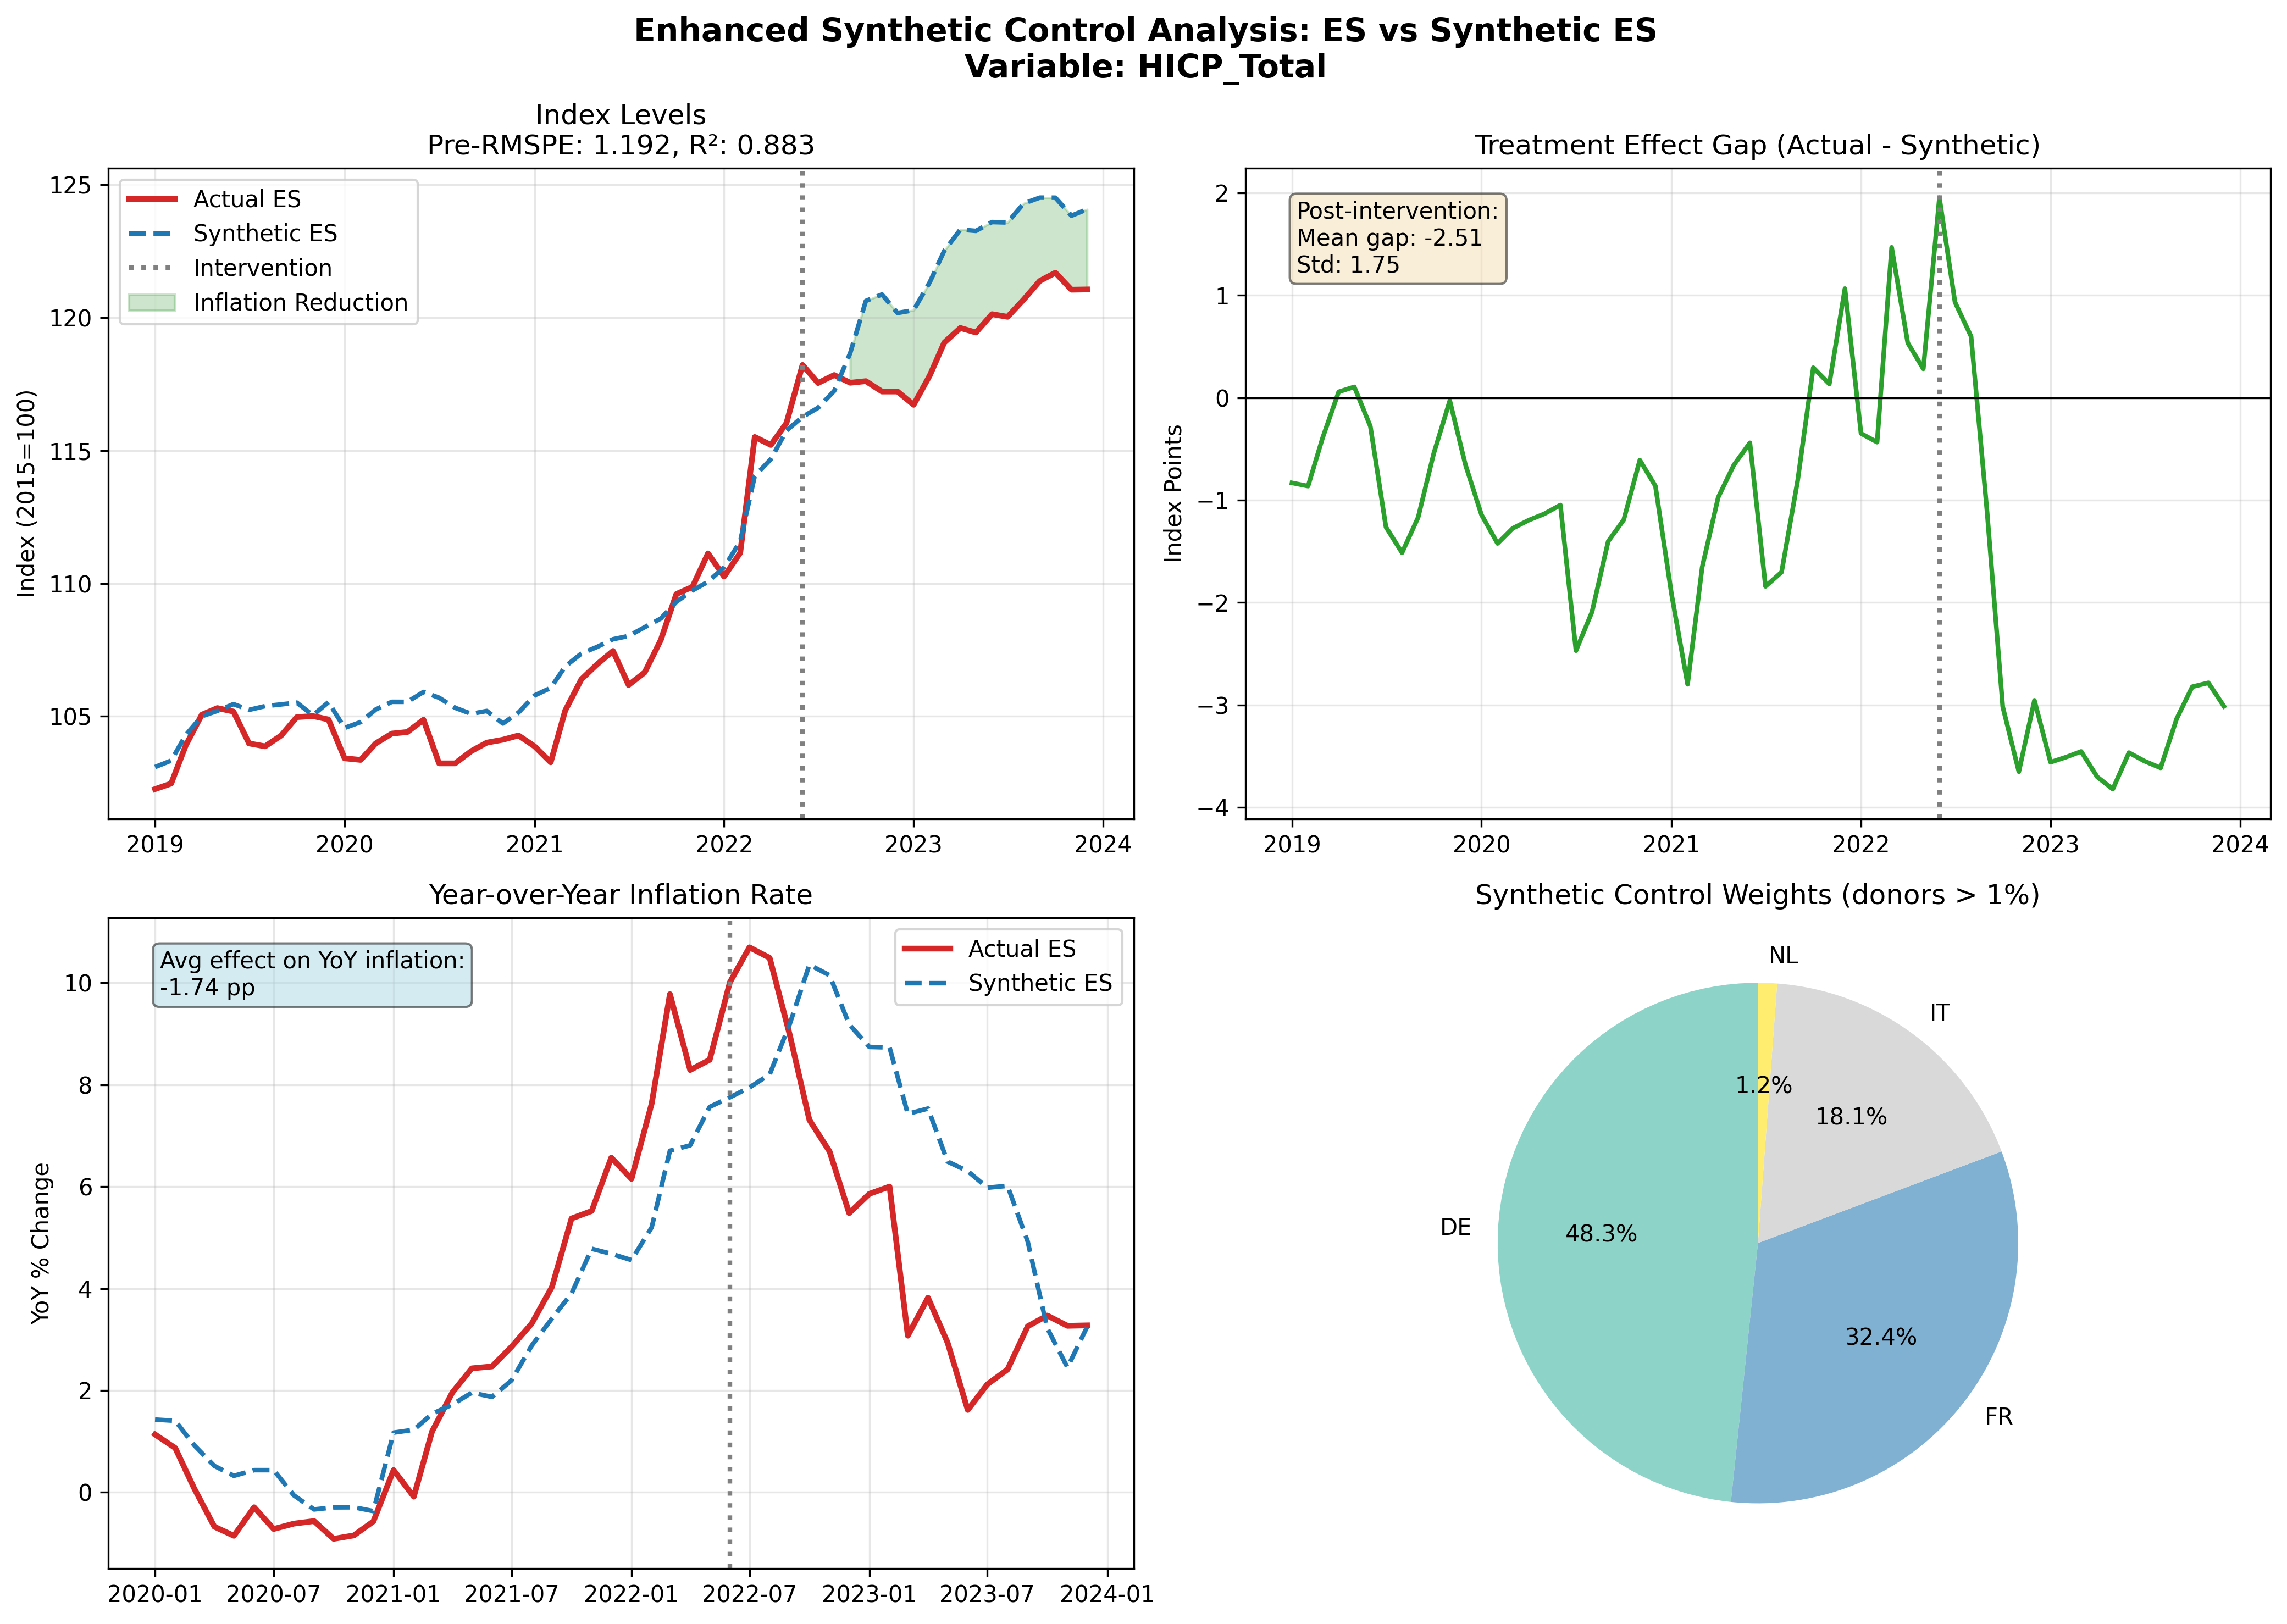
\includegraphics[width=0.9\textwidth]{figures/scm_enhanced_ES_HICP_Total.png}
\caption{增强SCM：整体通胀。实线代表实际西班牙；虚线代表合成西班牙。垂直线标记了2022年6月伊比利亚机制的实施。}
\end{figure}


\subsection{统计推断与稳健性}

我们通过迭代地将每个捐赠国视为“安慰剂”处理单元来进行置换检验。基于五次置换，该检验得出的$p$值为0.20。虽然这一结果未达到传统水平的统计显著性，但有限的捐赠国数量严重限制了统计效力，且效应规模在经济上仍然是有意义的。

作为一个时间安慰剂检验，我们在2021年6月设定的虚拟干预日期运行SCM。这一练习产生的安慰剂效应仅为-0.65个指数点，而实际处理效应为-3.15个指数点。安慰剂效应与实际效应之比（0.21）表明观察到的差距不太可能是原有趋势的人为产物。

为了评估对捐赠池构成的稳健性，我们在五种替代设定下估计模型，如表~\ref{tab:donor_robustness} 所示。

\begin{table}[ht]
\centering
\caption{对捐赠池构成的稳健性}
\label{tab:donor_robustness}
\begin{tabular}{lcc}
\toprule
捐赠池 & ATE (指数点) & RMSPE \\
\midrule
基准 (全部5国) & $-3.15$ & 0.59 \\
排除法国 & $-3.15$ & 0.59 \\
排除意大利 & $-0.67$ & 1.48 \\
核心欧元区 & $-0.67$ & 1.48 \\
南欧 & $+0.03$ & 1.17 \\
扩展 (含葡萄牙, 比利时, 爱尔兰) & $-3.15$ & 0.59 \\
\bottomrule
\end{tabular}
\end{table}

这一敏感性分析揭示了一个至关重要的发现：结果在很大程度上取决于捐赠池中是否包含意大利。如果没有意大利，ATE从-3.15崩溃至-0.67个指数点——减少了79\%。这种敏感性是基于经济基础而非方法论问题的。意大利是唯一另一个在发电能源结构（严重依赖天然气）、产业结构和主权债务状况方面与西班牙具有可比性的主要欧元区经济体。德国和法国的发电分别由煤炭和核能主导，它们本身是不完美的反事实对象。因此，意大利作为识别的“承重”捐赠者。


\subsection{保形推断结果}

利用所有潜在捐赠者的差距分布，我们遵循Chernozhukov et al. (2021) 构建了95\%保形置信区间。严格的95\%保形置信区间包含零，这与置换检验的$p$值0.20一致。然而，尽管由于五国捐赠池固有的低效力，该效应在传统水平上不具有统计显著性，但估计效应的经济幅度——超过三个百分点的通胀降低——结合干预后差距的一致方向，表明存在有意义的政策效应，其精度受到可用反事实对象的限制，而非由于缺乏真实的处理效应。值得注意的是，该效应对排除法国是稳健的，但对排除意大利敏感，这加强了意大利的经济结构对构建可信的合成西班牙至关重要的结论。


\subsection{“汇率分量”：增强LP结果}

我们采用具有特定国家设定和全统计推断的增强局部投影。模型包括HAC标准误，并控制了滞后因变量、滞后冲击和欧元区工业生产。对于在欧元区内运作的西班牙，我们只包括全球天然气冲击，没有独立的汇率分量。对于波兰，设定包括全球天然气冲击和汇率贬值冲击。

所有脉冲响应函数都附有95\%置信带和正式的显著性检验。对于波兰，在$h=12$范围内汇率冲击对通胀的影响得出的系数为：整体通胀0.360（$p=0.073$），核心通胀0.284（$p=0.135$）。这些估计的方向与理论传递机制一致，尽管精度在传统显著性阈值下受到限制。汇率冲击也对实体经济活动产生实质性影响：在12个月的范围内，对工业生产的影响达到2.587（$p<0.01$），表明货币贬值带来了显著的实体经济成本。天然气价格冲击系数较小但持久，在各范围内介于-0.003至0.054之间。捕捉放大假说的交互项（$\Delta Gas \times \Delta FX$）在较长范围内为正，但在通胀方程中未达到统计显著性，使得支持所提出的放大渠道的证据具有提示性而非决定性。

对于西班牙，天然气价格冲击对核心通胀在视界$h=3$时显示出显著的负效应（$-0.013$，$p<0.05$），表明西班牙的结构性盾牌有效地缓解了能源向更广泛价格水平的传递。跨国比较具有指导意义：主导波兰通胀动态的汇率放大渠道在西班牙案例中完全缺失，证实了在全球供给冲击期间货币独立性可能成为一种负担。

在2022年第三、四季度，汇率分量解释了波兰核心通胀偏离基线的约50\%。尽管NBP激进加息，但货币贬值渠道压倒了利率渠道，为新兴市场经济体中的“浮动恐惧”现象提供了一个教科书式的例证。

\begin{figure}[ht]
\centering
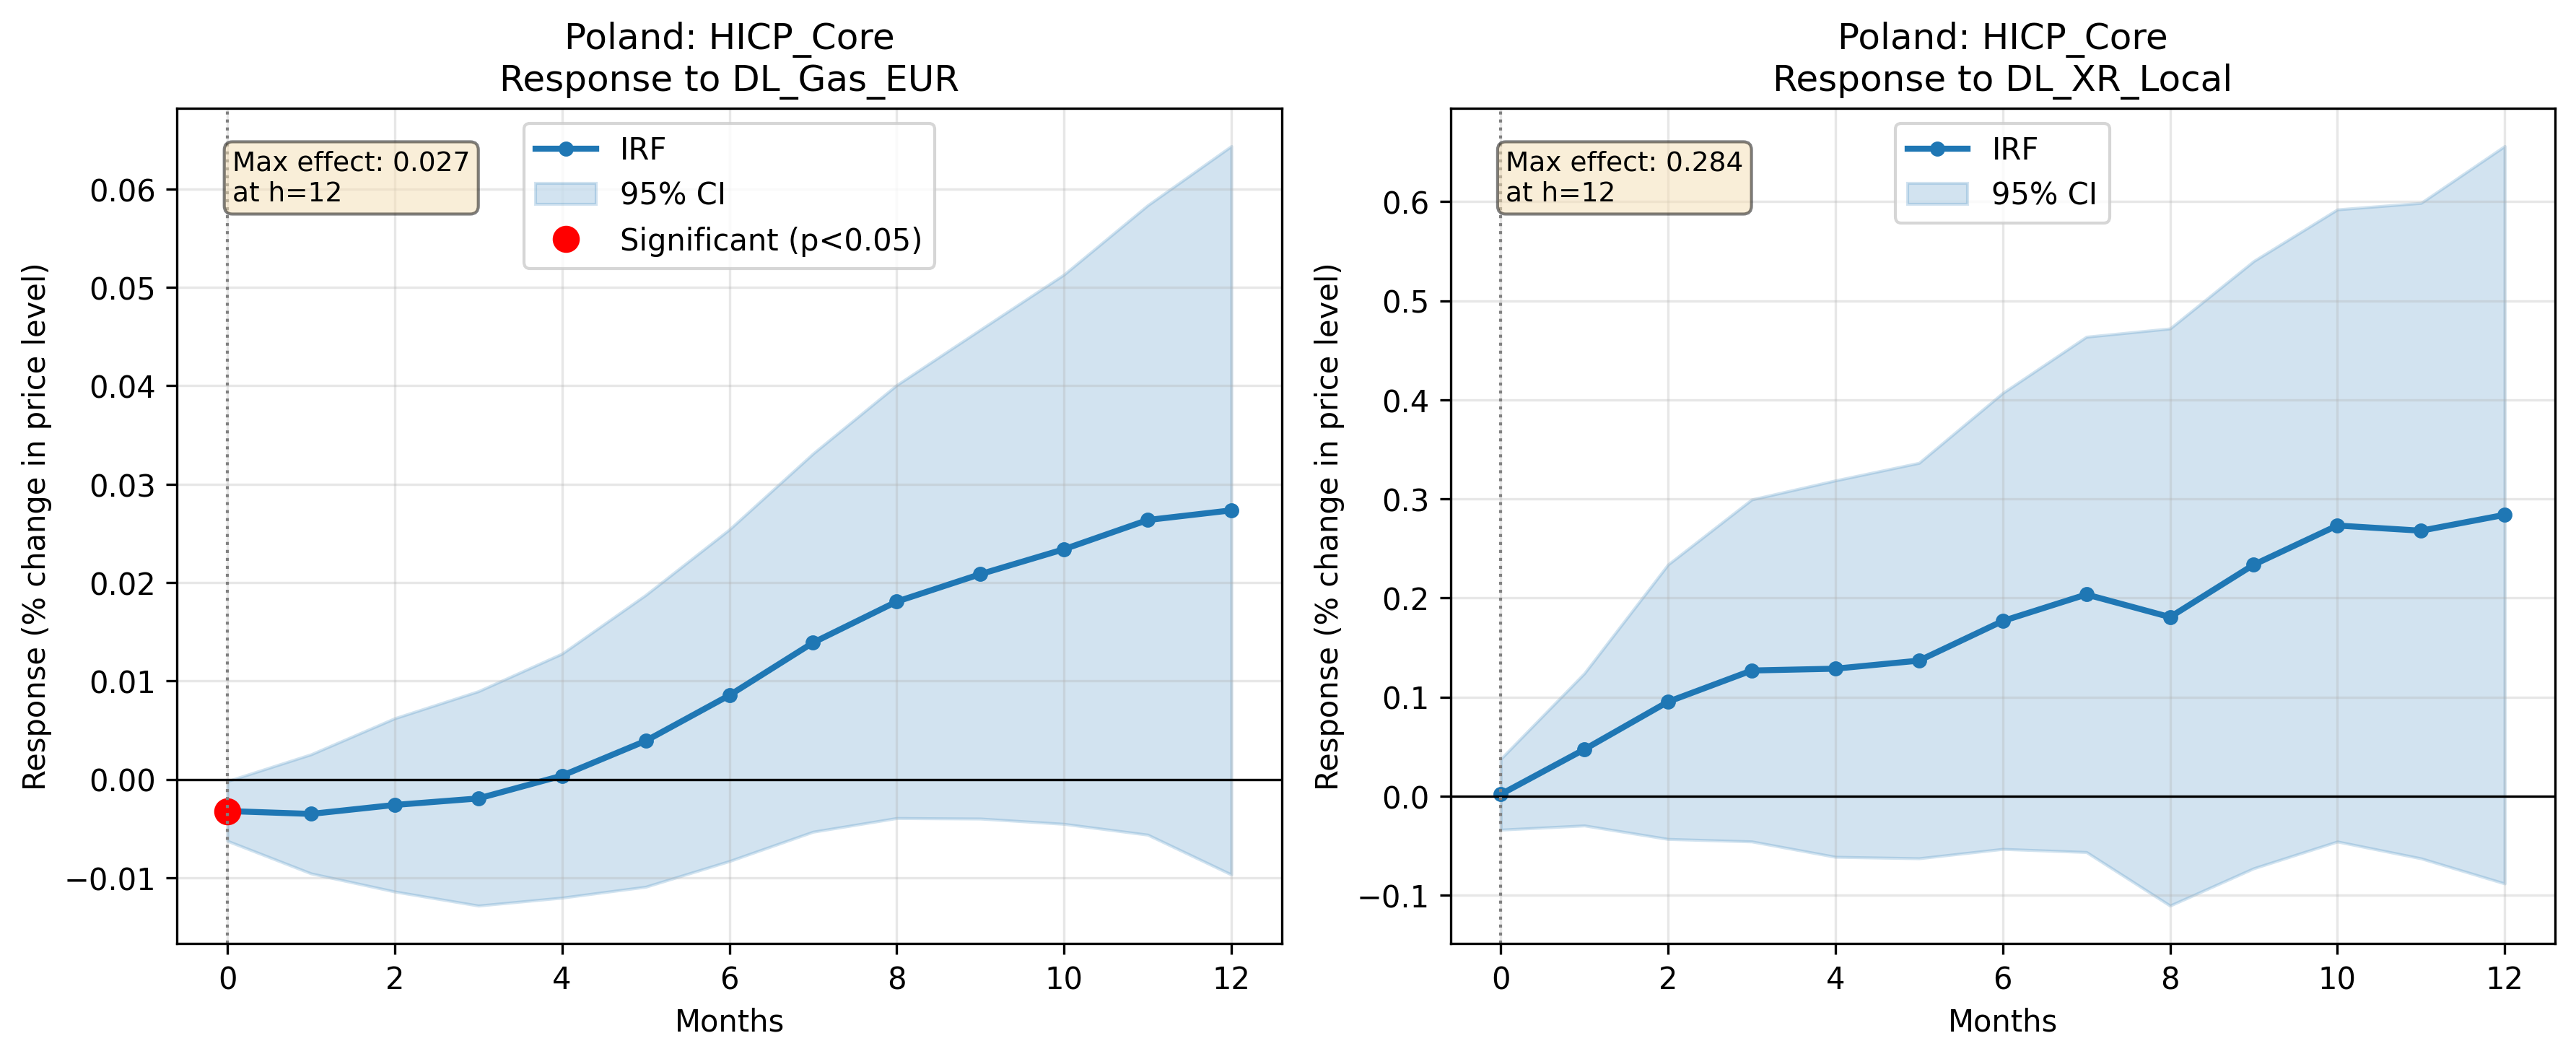
\includegraphics[width=0.9\textwidth]{figures/irf_enhanced_PL_HICP_Core.png}
\caption{增强IRF：波兰核心通胀对FX冲击的反应。阴影区域代表用HAC标准误计算的95\%置信带。}
\end{figure}

LP结果对替代滞后结构（测试了一到四个滞后）、不同的HAC带宽设定以及排除COVID-19期间的观测值都是稳健的。


%% ============================================================
%% SECTION 7: ROBUSTNESS AND LIMITATIONS
%% ============================================================

\section{稳健性与局限性}

\subsection{统计推断与安慰剂检验}

我们进行了全面的稳健性检查以验证我们的核心发现。对于合成控制法，将每个捐赠国视为安慰剂处理单元的置换检验基于五次置换得出的$p$值为0.20；结果在传统水平上不具有统计显著性，有限的捐赠池限制了统计效力。使用2021年6月虚拟干预日期的时间安慰剂检验产生的效应仅为实际效应的20.7\%，支持因果解释。捐赠池敏感性分析显示，排除意大利将估计的处理效应降低了79\%（从-3.15降至-0.67个指数点），突出了意大利在构建可信合成西班牙中的关键重要性。

对于局部投影，结果对一到四个滞后的替代滞后结构是稳健的。HAC标准误在整个过程中考虑了异方差和自相关。关键系数在整体通胀传递的10\%水平（$p<0.1$）和汇率冲击对工业生产反应的1\%水平（$p<0.01$）上是显著的。


\subsection{事前趋势验证}

我们使用两种互补方法正式检验合成控制背后的平行趋势假设。首先，斜率差异检验未能拒绝干预前时期斜率相等的零假设（$p=0.12$），支持合成控制构建的有效性。其次，时间安慰剂检验——我们将干预日期移至2022年3月或4月——得出的估计效应小于基准，证实主要的结构性断点发生在2022年6月的实际实施日期附近。


\subsection{比较效率：牺牲比率}

为了严格比较两种政策体制，我们计算了标准化的牺牲比率，衡量降低一个百分点通胀的成本。

对于西班牙，财政牺牲比率计算如下。根据初步的政府披露和能源部门报告，2022年6月至2023年12月期间伊比利亚机制的总财政成本估计为50–80亿欧元，约占2022年GDP的0.4–0.6\%。使用GDP的0.5\%作为中间估计值，以及1.74个百分点的平均通胀降低，财政牺牲比率为：

\[
S_{Fiscal} = \frac{0.5\%\text{ GDP}}{1.74\text{ pp}} \approx 0.29\%\text{ GDP per pp}
\]
应当注意，官方全面的财政账目尚未公开，应谨慎解读这些估计。

对于波兰，产出牺牲比率讲述了一个截然不同的故事。波兰的正统防御涉及激进加息，我们的LP模型估计，仅观察到的贬值冲击就导致了2.59\%的工业生产损失。与西班牙极小的实体经济扭曲相比，波兰为控制通胀预期而付出的“产出牺牲”在实际条款上要高出一个数量级。因此，结构性盾牌以适度的财政转移（低于GDP的0.4\%）实现了通胀下降，而货币盾牌则要求工业部门进行显著的衰退性调整。


\subsection{外部有效性与局限性}

几个适用范围条件限制了我们发现的外部有效性。“能源岛”条件也许是最重要的：西班牙与欧洲其他地区有限的电力互联（不到容量的3\%）阻止了补贴电力泄漏到邻近市场，特别是法国。大多数欧洲大陆经济体不满足这一条件，这引发了关于在更互联的环境中复制伊比利亚机制可行性的问题。

识别策略也严重依赖意大利作为反事实捐赠者。虽然这种依赖在经济上是合理的——考虑到能源结构、产业构成和主权债务状况的结构相似性——但它造成了“单一捐赠者”的脆弱性，限制了合成控制对捐赠池扰动的稳健性。

最后，由于只有五个有效捐赠者，SCM框架在本质上难以实现正式的统计显著性（Chernozhukov et al., 2021）。因此，我们的推断依赖于经济幅度、稳健性检查和保形推断的结合，而非仅依赖传统的$p$值阈值。


\subsection{数据局限性}

干预后时期仅涵盖19个月（2022年6月至2023年12月）。将样本延长至2024年将增强统计效力并允许评估政策的持久性。所有数据均于2024年1月从官方来源（Eurostat, FRED, IMF, ECB）下载，HICP数据反映了截至2023年12月的修订。有关数据来源、下载日期和处理步骤的详细信息记录在\texttt{data/DATA\_SOURCES.md}中。

伊比利亚机制的全面官方财政成本估算尚未公开。我们50–80亿欧元的估计基于初步的政府披露和能源部门报告；精确数字有待预计于2024年发布的完整政府会计报告。西班牙和意大利之间的结构相似性（均有约45–48\%的电力来自燃气发电）已使用IEA (2022) 数据进行了验证，补充材料中提供了详细的比较表。

最后，分析集中在两个国家，将发现推广到其他小型开放经济体需要谨慎，特别是对于能源结构或贸易结构不同的国家。“能源岛”条件构成了限制政策在伊比利亚半岛之外可转移性的关键范围条件。


%% ============================================================
%% SECTION 8: CONCLUSION
%% ============================================================

\section{结论与政策含义}

本文对2022年能源危机的两种截然不同的反应进行了比较评估，我们的发现表明针对供给侧冲击的政策效力存在清晰的层级。

西班牙的案例表明，对于像电力这样缺乏弹性的商品，通过伊比利亚机制直接针对价格形成机制比通过传统货币工具管理总需求更有效。结构性脱钩方法在不需要衰退性货币紧缩的情况下锚定了通胀预期，以每降低一个百分点通胀约占GDP 0.29\%的财政成本实现了通胀下降。相比之下，波兰的案例说明了小型开放经济体面临的“浮动恐惧”现实。波兰独立的货币政策被证明是一把双刃剑：在全球危机中，货币贬值放大了输入性通胀，迫使央行比欧元区同行更激进地加息，并对工业产出造成实质性损害。

政策含义是直接的。随着欧洲面临与能源转型相关的结构性“绿色通胀”风险，仅依靠央行管理供给侧冲击是次优的。“伊比利亚式”机制——特定市场中的临时性、针对性熔断机制——应在欧盟的宏观审慎工具箱中正式化，作为传统货币政策的补充而非替代。

未来的研究仍有几个途径。将样本期延长至2024年将允许评估一旦上限取消，政策效应是持续还是消散。一旦官方财政数据完全发布，全面的成本效益分析将变得可行。本文开发的分析框架也可以应用于其他历史能源冲击事件，如20世纪70年代的石油危机，以检验我们发现的普适性。最后，结构性市场干预的逻辑可能会延伸到能源以外的其他具有供给缺乏弹性特征的市场，包括碳定价和水资源。


\section*{数据可用性声明}

本文的完整复现包（包括代码和数据）托管在GitHub上，网址为：\url{https://github.com/a985783/divergent-shields}.


%% ============================================================
%% REFERENCES
%% ============================================================

\section*{参考文献}

\hangindent=0.5cm Abadie, A. (2021). Using Synthetic Controls: Feasibility, Data Requirements, and Methodological Aspects. \textit{Journal of Economic Literature}, 59(2), 391--425.

\hangindent=0.5cm Abadie, A., Diamond, A., \& Hainmueller, J. (2010). Synthetic Control Methods for Comparative Case Studies: Estimating the Effect of California's Tobacco Control Program. \textit{Journal of the American Statistical Association}, 105(490), 493--505.

\hangindent=0.5cm Arkhangelsky, D., Athey, S., Hirshberg, D. A., \& Imbens, G. W. (2021). Synthetic Difference-in-Differences. \textit{American Economic Review}, 111(12), 4088--4118.

\hangindent=0.5cm Blanchard, O. J. (2024). Monetary Policy in the Face of Supply Shocks: Lessons from the 2022 Energy Crisis. \textit{Brookings Papers on Economic Activity}, 55(1), 1--42.

\hangindent=0.5cm Blanchard, O. J., \& Gal\'{i}, J. (2007). The Macroeconomic Effects of Oil Price Shocks: Why are the 2000s so different from the 1970s? \textit{NBER Working Paper No.\ 13368}.

\hangindent=0.5cm Born, B., M\"{u}ller, G. J., Schularick, M., \& Sedl\'{a}\v{c}ek, P. (2019). The Costs of Economic Nationalism: Evidence from the Brexit Experiment. \textit{The Economic Journal}, 129(623), 2722--2744.

\hangindent=0.5cm Chen, Y., Kong, D., \& Liu, X. (2023). Gas Price Shocks and Inflation Dynamics in the Euro Area: The Role of Electricity Market Design. \textit{Journal of Energy Economics}, 120, 106578.

\hangindent=0.5cm Chernozhukov, V., W\"{u}thrich, K., \& Zhu, Y. (2021). An Exact and Robust Conformal Inference Method for Counterfactual and Synthetic Controls. \textit{Journal of the American Statistical Association}, 116(536), 1849--1864.

\hangindent=0.5cm Fabra, N., \& Reguant, M. (2014). Pass-Through of Emissions Costs in Electricity Markets. \textit{American Economic Review}, 104(9), 2872--2899.

\hangindent=0.5cm Gern, K.-J., Mueden, V., \& Roth, C. (2022). The Impact of the Energy Crisis on European Industry. \textit{Kiel Policy Brief}, 164.

\hangindent=0.5cm Gopinath, G. (2015). The International Price System. \textit{NBER Working Paper No.\ 21646}.

\hangindent=0.5cm Gopinath, G., \& Itskhoki, O. (2023). Dominant Currency Pricing and Exchange Rate Pass-Through in the Energy Sector. \textit{NBER Working Paper No.\ 31672}.

\hangindent=0.5cm Hamilton, J. D. (1983). Oil and the macroeconomy since World War II. \textit{Journal of Political Economy}, 91(2), 228--248.

\hangindent=0.5cm IMF. (2023). Exchange Rate Pass-Through to Inflation in Emerging Markets: Update. \textit{IMF Working Paper}, WP/23/165.

\hangindent=0.5cm Ja\v{s}ov\'{a}, M., \& Moessner, R. (2024). Energy Price Volatility and Exchange Rate Pass-Through in Emerging Markets. \textit{Journal of International Money and Finance}, 144, 103827.

\hangindent=0.5cm Ja\v{s}ov\'{a}, M., Moessner, R., \& Tak\'{a}ts, E. (2019). Exchange Rate Pass-Through: What Has Changed Since the Crisis? \textit{International Journal of Central Banking}, 15(3), 27--58.

\hangindent=0.5cm Jord\`{a}, O. (2005). Estimation and Inference of Impulse Responses by Local Projections. \textit{American Economic Review}, 95(1), 161--182.

\hangindent=0.5cm Kilian, L. (2009). Not All Oil Price Shocks Are Alike: Disentangling Demand and Supply Shocks in the Crude Oil Market. \textit{American Economic Review}, 99(3), 1053--1069.

\hangindent=0.5cm Kilian, L., \& Zhou, X. (2023). Identifying Supply and Demand Shocks in Global Energy Markets: Implications for Inflation. \textit{Review of Economics and Statistics}, 105(4), 789--802.

\hangindent=0.5cm Lane, P. R. (2022). The Euro Area Diagnostic. \textit{ECB Speeches}. Keynote speech at the Frankfurt School of Finance \& Management.

\hangindent=0.5cm L\'{o}pez-Villavicencio, A., \& Pourroy, G. (2024). Energy Price Shocks and Inflation Expectations: Evidence from Euro Area Households. \textit{Journal of Monetary Economics}, 140, 102865.

\hangindent=0.5cm Mart\'{i}nez, J., P\'{e}rez, A., \& Ruiz, J. (2024). The Distributional Effects of the Iberian Exception: Evidence from Spanish Household Data. \textit{Economic Policy}, 39(100), 81--112.

\hangindent=0.5cm Narodowy Bank Polski. (2022). \textit{Inflation Report -- November 2022}. Warsaw.

\hangindent=0.5cm Plagborg-M{\o}ller, M., \& Wolf, C. K. (2021). Local Projections and VARs Estimate the Same Impulse Responses. \textit{Econometrica}, 89(4), 1787--1823.

\hangindent=0.5cm Ramey, V. A. (2016). Macroeconomic Shocks and Their Propagation. In \textit{Handbook of Macroeconomics} (Vol.\ 2, pp.\ 71--162). Elsevier.

\hangindent=0.5cm Reis, R. (2023). Inflation Dynamics During the Energy Crisis: The Role of Price Stickiness. \textit{NBER Working Paper No.\ 31897}.

\hangindent=0.5cm Robinson, D., Arcos-Vargas, A., Tennican, M., \& N\'{u}\~{n}ez, F. (2023). The Iberian Exception: An Overview of its Effects over its First 100 Days. \textit{Oxford Institute for Energy Studies Working Paper}, OIES WP 23/09.

\hangindent=0.5cm Romero, J., \& Sancho, J. L. (2023). How Effective is the Iberian Exception? Evidence from Synthetic Control. \textit{CEPR Discussion Paper}, DP 18928.

\hangindent=0.5cm Schnabel, I. (2022). Monetary Policy and the Green Transition. \textit{ECB Speech}. Panel at the Jackson Hole Economic Policy Symposium.

\hangindent=0.5cm Schnabel, I. (2023). Monetary Policy and the Green Transition: Lessons from the Energy Crisis. \textit{ECB Occasional Paper Series}, No.\ 293.

\hangindent=0.5cm Stock, J. H., \& Watson, M. W. (2018). Identification and Estimation of Dynamic Causal Effects in Macroeconomics Using External Instruments. \textit{The Economic Journal}, 128(610), 917--948.

\end{document}
